

\section{Alternative parent selection}
 This section will discuss two alternative forms of parent selection: tournament selection and fitness proportionate selection. 
 
 \subsection{Fitness proportionate selection}
 The fitness proportionate selection method assigns to each individual a probability of selection that is directly proportional to its fitness value. This is summed up in formula \ref{eq:fitness_prop}. Because the fitness function is to be minimised, the fitness values are inverted prior to calculating the probabilities. 
 \begin{equation} \label{eq:fitness_prop}
 P(i) = \dfrac{\dfrac{1}{f_i}}{\sum\limits_{j=1}^\mu {\dfrac{1}{f_j}}}
 \end{equation}
 Next, Stochastic Universal Sampling (SUS) is used to select parents based on the probabilities obtained from \ref{eq:fitness_prop}.
 
 After some parameter tuning we performed some of the same benchmarks as in section \ref{sec:benchmarks}. Figure \ref{fig:fps_gen} shows the result of the 380-city benchmark. It is immediately clear that the fitness proportionate selection performs much worse than the previous selection method. A possible explanation would be that the process with fitness proportionate selection often stagnates quite quickly because it tends to suffer from premature convergence. However, looking at the histogram in figure \ref{fig:fps_hist} there still seems to be a fairly large amount of variation in the population. It is more likely that the fitness values of the population are too close to each other, resulting in low selection pressure (because similar fitness values lead to similar selection probabilities and therefore low selection pressure).
 
 
  \begin{figure}[!]
\centering
\begin{subfigure}{0.45\textwidth}
  \centering
  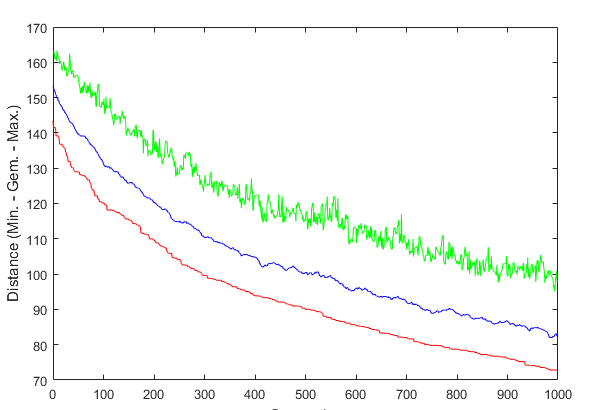
\includegraphics[width=1\textwidth]{../figures/question_5/FPS_off_gens.png}
      \caption{\textbf{Loop detection off}. \textbf{Best tour distance found: $\mathbf{72.79}$, computation time: 390 seconds}. } 
      \label{fig:fps_vraag5_off_gen}
\end{subfigure}
\hspace{0.05\textwidth}
\begin{subfigure}{0.45\textwidth}
  \centering
  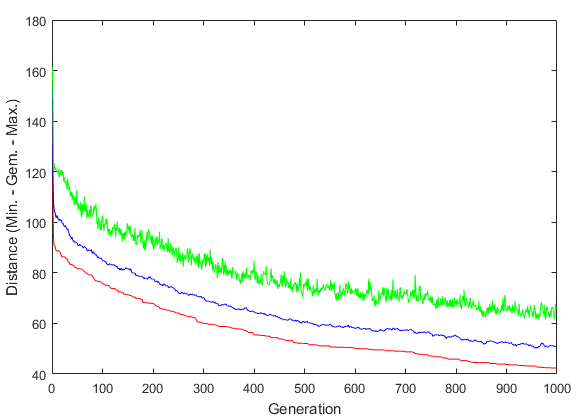
\includegraphics[width=1\textwidth]{../figures/question_5/FPS_on_gens.png}
      \caption{\textbf{Loop detection on}.  \textbf{Best tour distance found: $\mathbf{42.36}$, computation time: 431 seconds}.} 
      \label{fig:fps_vraag5_off_gen}
\end{subfigure}
\caption{The benchmark TSP problem \texttt{bcl380.tsp} with 380 cities is solved here using path representation with the following parameters: PR. MUT = $25\%$, PR. CROS = $60\%$ , ELITE = $5\%$. 200 individuals and 1000 generations.}
\label{fig:fps_gen}
\end{figure}

\begin{figure}[!]
\centering
 \scalebox{.5}{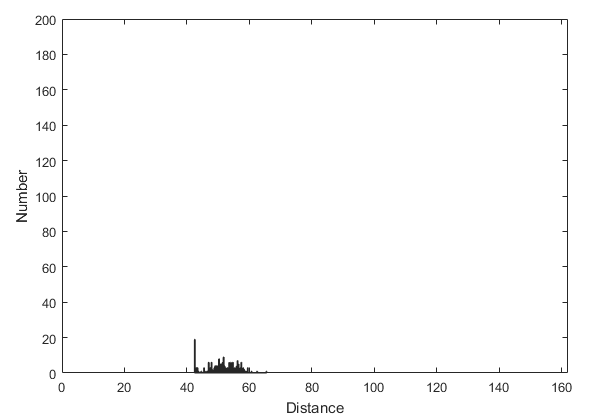
\includegraphics{../figures/question_5/FPS_hist.png}}
 
 \caption{Histogram at 1000 generations using path representations with fitness proportionate selection.}
 \label{fig:fps_hist}
\end{figure}


 \subsection{Tournament selection}
 Tournament selection selects parents by randomly choosing groups of n members of the population. From each group the individual with the best fitness value is selected as a parent. This continues until enough parents have been selected. For a full explanation we refer to \cite{handboek}.
 
 To test this selection mechanism the same method as in the previous section is used. From \ref{fig:tour_gen} it is clear that tournament selection does offer an improvement over the default rank selection. Worth noting is that tournament selection performs just as well with loop detection disabled as rank selection does with it enabled. A reason for this increased performance might be that tournament selection (with the right tournament size) strikes a good balance between selection pressure and sufficient probability for less fit members to survive, giving the algorithm greater chances of abandoning local optima that are not near the global optimum.
 
 A downside to the tournament selection is that after a large amount of generations, the variety in the population becomes extremely low. Figure \ref{fig:tourn_hist} shows over half of the population sitting at the same fitness (and thus likely representing the same tour). This reduces the effectiveness of the algorithm and might cause it to get stuck in a local optimum after all. The use of mechanisms to increase population diversity (e.g. supbpopulations) might give further improvements to the algorithm.
 
   \begin{figure}[!]
\centering
\begin{subfigure}{0.45\textwidth}
  \centering
  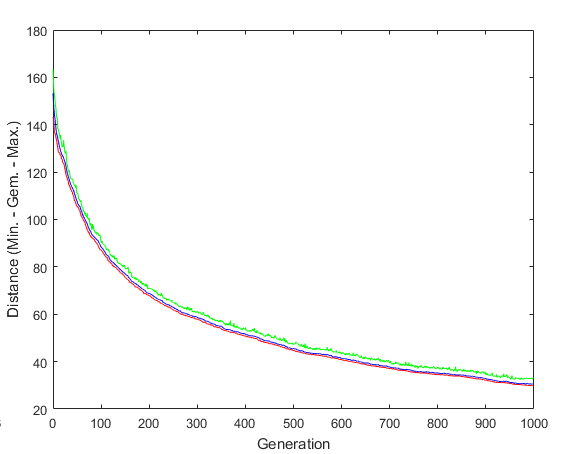
\includegraphics[width=1\textwidth]{../figures/question_5/tournament_off_gen.png}
      \caption{\textbf{Loop detection off}. \textbf{Best tour distance found: $\mathbf{26.79}$, computation time: 412 seconds}. } 
      \label{fig:tourn_vraag5_off_gen}
\end{subfigure}
\hspace{0.05\textwidth}
\begin{subfigure}{0.45\textwidth}
  \centering
  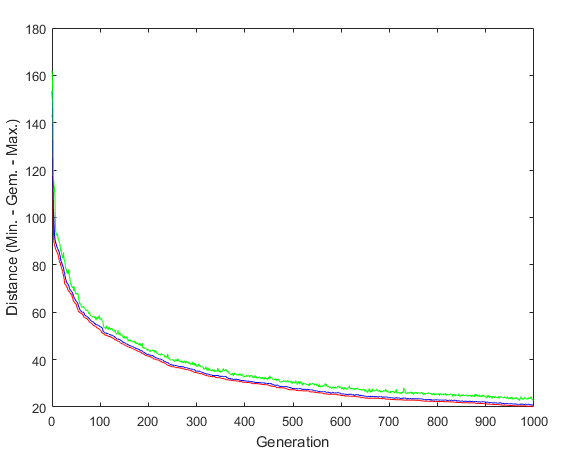
\includegraphics[width=1\textwidth]{../figures/question_5/tournament_on_on.png}
      \caption{\textbf{Loop detection on}.  \textbf{Best tour distance found: $\mathbf{20.21}$, computation time: 441 seconds}.} 
      \label{fig:tourn_vraag5_off_gen}
\end{subfigure}
\caption{The benchmark TSP problem \texttt{bcl380.tsp} with 380 cities is solved here using path representation and tournament selection with the following parameters: PR. MUT = $20\%$, PR. CROS = $60\%$ , ELITE = $5\%$, TOURN. SIZE = 5. 200 individuals and 1000 generations.}
\label{fig:tour_gen}
\end{figure}


\begin{figure}[!]
\centering
 \scalebox{.5}{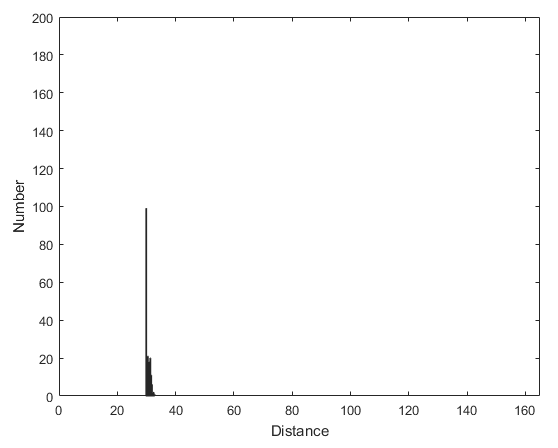
\includegraphics{../figures/question_5/tournament_off_hist.png}}
 
 \caption{Histogram at 1000 generations using path representations with tournament selection.}
 \label{fig:tourn_hist}
\end{figure}

\FloatBarrier